%% phase_N1_report.tex
%% Self-contained report on Phase N1: Clean European Temporal EOC Study
%% Compile with: pdflatex phase_N1_report.tex
%%
\documentclass[11pt,a4paper]{article}

\usepackage{amsmath, amssymb, amsthm}
\usepackage{booktabs}
\usepackage{graphicx}
\usepackage{geometry}
\usepackage{hyperref}
\usepackage{microtype}
\usepackage{xcolor}
\usepackage{caption}
\usepackage{subcaption}
\usepackage{enumitem}

\geometry{margin=2.5cm}

\hypersetup{
  colorlinks=true, linkcolor=blue!60!black,
  citecolor=blue!60!black, urlcolor=blue!60!black
}

% convenience
\newcommand{\Lp}[1]{L^{#1}}
\newcommand{\Nx}{N_x}
\newcommand{\Nt}{N_t}
\newcommand{\dt}{\Delta t}
\newcommand{\bigo}[1]{\mathcal{O}(#1)}
\newcommand{\eps}{\varepsilon}

% ------------------------------------------------------------------
\title{\textbf{Phase N1: Clean European Temporal Convergence Study}\\
       \large V2 Ultraweak DPG Solver — European Call Option}
\author{dpg-finance project}
\date{2026-05-28 \quad (commit \texttt{6f55973})}
% ------------------------------------------------------------------

\begin{document}
\maketitle
\tableofcontents
\bigskip

% ==================================================================
\section{Objective}
% ==================================================================

The goal of Phase~N1 is to isolate and measure the \emph{temporal}
discretization error of the V2 solver independently of its spatial
discretization error.  Specifically, we seek to verify that the
backward Euler time-stepping scheme, combined with the ultraweak DPG
spatial discretization, achieves the theoretically expected
first-order convergence rate
\[
  \|u_h^{N_t} - u_{\rm exact}\|_{L^2} = \bigo{\dt}, \qquad \dt = T/\Nt,
\]
in the regime where the temporal error dominates the spatial error.

% ==================================================================
\section{Mathematical Formulation}
% ==================================================================

\subsection{Black-Scholes PDE in log-price coordinates}

Under the log-price change of variables $x = \log(S/K)$ and
backward time $\tau = T - t$, the European call option price
$u(x,\tau)$ satisfies
\begin{equation}\label{eq:bs-pde}
  \frac{\partial u}{\partial \tau}
  - \underbrace{\frac{\sigma^2}{2}}_{=:\,\mathrm{diff}}\,
    \frac{\partial^2 u}{\partial x^2}
  - \underbrace{\!\left(r - \frac{\sigma^2}{2}\right)}_{=:\,b}\!
    \frac{\partial u}{\partial x}
  + r\,u = 0,
  \qquad (x,\tau)\in\mathbb{R}\times(0,T],
\end{equation}
with initial condition (payoff at expiry)
\[
  u(x,0) = K\max\!\bigl(e^x - 1,\,0\bigr)
\]
and the exact analytical solution given by the Black-Scholes formula
\[
  u_{\rm exact}(x,\tau)
    = K e^x N(d_1) - K e^{-r\tau} N(d_2),
\]
where $d_{1,2} = \bigl(x + (r \pm \tfrac{1}{2}\sigma^2)\tau\bigr)
/ (\sigma\sqrt{\tau})$ and $N(\cdot)$ is the standard normal CDF.

\subsection{Ultraweak DPG first-order system (V2)}

Equation~\eqref{eq:bs-pde} is rewritten as a first-order system by
introducing the auxiliary flux variable
$\boldsymbol{\sigma}_h = \mathrm{diff}\,\nabla u$.  After backward
Euler time discretization with step size $\dt$, the per-step problem
reads: given $u^n$, find $(u^{n+1},\boldsymbol{\sigma}^{n+1},
\hat{u},\hat{f})\in\mathcal{U}_h\times\boldsymbol{\Sigma}_h\times
\hat{\mathcal{U}}_h\times\hat{\mathcal{F}}_h$ such that

\begin{align}
  -b\,(u,\nabla v)
  + (\boldsymbol{\sigma},\nabla v)
  + \tfrac{1}{\dt+r}\,(u,v)
  + \langle \hat{f}, v \rangle
  &= \tfrac{1}{\dt}(u^n,\,v),
  \label{eq:uw-row1}\\[4pt]
  (u,\nabla{\cdot}\,\boldsymbol{\tau})
  + \tfrac{1}{\mathrm{diff}}\,(\boldsymbol{\sigma},\boldsymbol{\tau})
  + \langle \hat{u},\,\boldsymbol{\tau}{\cdot}\mathbf{n}\rangle
  &= 0,
  \label{eq:uw-row2}
\end{align}
for all test functions $(v,\boldsymbol{\tau})$ in the enriched test
space, chosen optimally with respect to the adjoint-graph
test norm.

\paragraph{Finite element spaces.}
Trial spaces use $p=2$, $\delta p = 1$ (enrichment):
\begin{itemize}[noitemsep]
  \item $u_h \in L^2_{p-1}(\Omega_h)$ (piecewise linear, discontinuous),
  \item $\boldsymbol{\sigma}_h \in [L^2_{p-1}(\Omega_h)]^2$,
  \item $\hat{u}_h \in H^1_{\rm Trace}(\partial\mathcal{T}_h)$
         (H1 boundary traces, order $p$),
  \item $\hat{f}_h \in \mathrm{RT}_{\rm Trace}(\partial\mathcal{T}_h)$
         (RT boundary flux traces, order $p-1$).
\end{itemize}
The test spaces are $H^1$ of order $p+\delta p = 3$ and
$H(\mathrm{div})$ of order $p+\delta p-1=2$.

\paragraph{Preconditioner.}
A block-diagonal preconditioner is applied with four independent
AMG (BoomerAMG) sub-solvers, one per trial block.
Prior to Phase~N1, block~3 (RT flux traces) used HypreAMS,
which failed for $\Nx > 300$ on quasi-1D meshes;
this was replaced by HypreBoomerAMG (see Section~\ref{sec:solver-fix}).

% ==================================================================
\section{Experimental Design}
% ==================================================================

\subsection{Design principle: spatial floor}

A clean temporal convergence study requires the spatial error to be
\emph{well below} the temporal error throughout the sweep.  Concretely,
if $\eps_{\rm spatial}$ denotes the spatial discretization floor and
$C_t$ is the temporal error constant, we need
\[
  \eps_{\rm spatial} \;\ll\; C_t\,\dt_{\rm min},
  \qquad \dt_{\rm min} = T/\Nt^{\rm max}.
\]
We fix the spatial mesh and vary only $\Nt$.

\subsection{Choice of domain and mesh}

\paragraph{Domain $[-6,6]$ with $\Nx=512$ (rejected).}
Initial experiments used domain $[-6,6]$ with $\Nx=512$.  Although the
solver converges (after the preconditioner fix), the exact call price
at $x = 6$ is $K e^6 - K e^{-r T} \approx 40\,245$, making the
absolute $L^2$ norm over $[-6,6]$ very large.  The spatial floor
measured by a fine-time reference run ($\Nt=1000$) was
$\eps_{\rm spatial} = 0.307$, while the temporal error at
$\Nt=512$ is $\bigo{0.014}$.  Since $0.307 \gg 0.014$, the spatial
floor dominates the entire sweep and the apparent temporal convergence
rate is $\approx 0.66$, below the acceptable range.

\paragraph{Domain $[-3,3]$ with $\Nx=256$ (adopted).}
The standard domain used throughout the spatial convergence
studies (Phase~A) has $[-3,3]$, $\Nx=256$, mesh size
$h = 6/256 = 0.02344$.  From the V2 spatial convergence table
(computed with $\Nt=5\,000$), the spatial floor is
$\eps_{\rm spatial} = 0.01535$.  With $\Nt=8$ (coarsest sweep point,
$\dt=0.125$), the temporal error satisfies $C_t\,\dt \approx 0.045$,
giving a temporal-to-floor ratio of $\approx 3$, sufficient for
visible first-order convergence.

\subsection{Parameters}

\begin{center}
\begin{tabular}{ll}
\toprule
Parameter & Value \\
\midrule
Option type         & European call \\
Strike $K$          & 100 \\
Risk-free rate $r$  & 0.05 \\
Maturity $T$        & 1 \\
Log-price domain    & $[-3,\,3]$ \\
Spatial mesh        & $\Nx = 256$ uniform elements \\
Mesh size           & $h = 0.02344$ \\
Spatial floor $\eps_{\rm spatial}$ & $0.01535$ (from $\Nt=5\,000$ reference) \\
Time steps swept    & $\Nt \in \{8,16,32,64,128,256,512\}$ \\
Volatilities        & $\sigma = 0.20$ (main) and $\sigma = 0.05$ (robustness) \\
MPI processes       & 4 \\
Solver              & PCG + block-diagonal BoomerAMG \\
\bottomrule
\end{tabular}
\end{center}

\subsection{Plateau flag}

A row is labeled as \emph{plateau} (flag~$= 1$) when
$\|u_h - u_{\rm exact}\|_{L^2} < 2\,\eps_{\rm spatial} = 0.0307$.
Pre-plateau rows (flag~$= 0$) are used to compute the fitted
temporal convergence rate.

\subsection{Preconditioner fix}\label{sec:solver-fix}

Before Phase~N1, the V2 solver used \texttt{HypreAMS} for the
RT\_Trace diagonal block of the block-diagonal preconditioner.
Testing revealed that \texttt{HypreAMS} fails silently for $\Nx > 300$
on quasi-1D meshes (512~elements$\,\times\,$1 element in the
transverse direction), producing 2\,000 non-converged CG iterations
per time step.  The fix is to replace \texttt{HypreAMS} with
\texttt{HypreBoomerAMG} for that block and raise the CG iteration
limit from 2\,000 to 5\,000.  All four blocks now use BoomerAMG.
This change is backward-compatible: results for previously tested
mesh sizes ($\Nx \le 256$) are unchanged.

% ==================================================================
\section{Results: \texorpdfstring{$\sigma = 0.20$}{sigma=0.20}}
% ==================================================================

\subsection{Full sweep data}

Table~\ref{tab:sigma020} shows the complete $L^2$ and
$L^\infty$ errors for $\sigma=0.20$.
The ATM price $u_h(0)$ is evaluated at the log-price $x=0$
(spot $S = K = 100$); the exact ATM call price is
$u_{\rm exact}(0,T) \approx 10.4506$.

\begin{table}[htbp]
\centering
\caption{Temporal convergence, $\sigma=0.20$, $\Nx=256$, domain $[-3,3]$.
  $\dagger$ = plateau (flag~1); excluded from pre-plateau EOC fit.}
\label{tab:sigma020}
\begin{tabular}{rr@{\;}lr@{\;}lr@{\;}lr}
\toprule
$\Nt$ & \multicolumn{2}{c}{$\dt$}
      & \multicolumn{2}{c}{$\|u_h - u_{\rm exact}\|_{L^2}$}
      & \multicolumn{2}{c}{EOC$_{L^2}$}
      & ATM error \\
\midrule
  8 & $1.250$&$\times 10^{-1}$ & $6.006$&$\times 10^{-2}$ & ---  & & $3.12\times10^{-2}$ \\
 16 & $6.250$&$\times 10^{-2}$ & $3.331$&$\times 10^{-2}$ & $0.85$ & & $3.57\times10^{-2}$ \\
 32 & $3.125$&$\times 10^{-2}$ & $1.827$&$\times 10^{-2}$ & $0.87$ &$\dagger$ & $2.89\times10^{-2}$ \\
 64 & $1.563$&$\times 10^{-2}$ & $1.045$&$\times 10^{-2}$ & $0.81$ &$\dagger$ & $2.37\times10^{-2}$ \\
128 & $7.813$&$\times 10^{-3}$ & $7.246$&$\times 10^{-3}$ & $0.53$ &$\dagger$ & $1.98\times10^{-2}$ \\
256 & $3.906$&$\times 10^{-3}$ & $7.432$&$\times 10^{-3}$ & $-0.04$ &$\dagger$ & $1.63\times10^{-2}$ \\
512 & $1.953$&$\times 10^{-3}$ & $1.036$&$\times 10^{-2}$ & $-0.48$ &$\dagger$ & $1.33\times10^{-2}$ \\
\midrule
\multicolumn{8}{l}{$\eps_{\rm spatial} = 0.01535$, spatial floor threshold $2\eps = 0.0307$} \\
\bottomrule
\end{tabular}
\end{table}

\subsection{Convergence analysis for \texorpdfstring{$\sigma=0.20$}{sigma=0.20}}

\paragraph{Pre-plateau convergence.}
The pre-plateau rows ($\Nt = 8$ and $\Nt = 16$, flag~0) give a
single measured EOC of $\mathbf{0.85}$, consistent with the
expected first-order rate of backward Euler.

Looking beyond the formal plateau threshold, the rows $\Nt = 32$
and $\Nt = 64$ (flag~1, but the $L^2$ error is still decreasing)
show EOC values of $0.87$ and $0.81$, respectively.  The $L^2$
error decreases monotonically from $6.0\times10^{-2}$ at
$\Nt=8$ through $1.0\times10^{-2}$ at $\Nt=64$, strongly
suggesting that the underlying temporal convergence rate is
$\bigo{\dt}$ over this entire range.

\paragraph{Plateau region ($\Nt \ge 128$).}
Beyond $\Nt=128$, the $L^2$ error reaches a minimum of
$\approx 7.2\times10^{-3}$ (below $\eps_{\rm spatial}$) and
then \emph{increases} back toward the spatial floor.  This
non-monotone behavior is characteristic of sign-opposite
interaction between the spatial and temporal errors: the
backward Euler dissipation partially cancels the DPG
spatial overestimation, reaching a cancellation minimum
at $\Nt \approx 128$--$256$, before temporal error vanishes
and the spatial floor dominates.

\paragraph{Remark on ATM error.}
The pointwise error at the ATM point ($x=0$) shows a minor
non-monotone excursion: it increases from $3.12\times10^{-2}$
($\Nt=8$) to $3.57\times10^{-2}$ ($\Nt=16$), then decreases
monotonically for all larger $\Nt$.  This behavior is a
known artifact of applying backward Euler to a problem with a
non-smooth initial condition (the call option payoff has a
kink at $x=0$): at very coarse time steps the specific
smoothing pattern of the BE method near $x=0$ is not
yet settled.  The global $L^2$ error, which averages over
the entire domain, \emph{is} monotone for the pre-plateau rows
and is the appropriate measure of temporal convergence rate.

% ==================================================================
\section{Results: \texorpdfstring{$\sigma = 0.05$}{sigma=0.05}
  (Convection-Dominated Regime)}
% ==================================================================

\subsection{Full sweep data}

Table~\ref{tab:sigma005} shows the sweep for $\sigma=0.05$.
For this volatility, $\mathrm{diff} = \sigma^2/2 = 0.00125$ and
the drift $b = r - \mathrm{diff} = 0.04875$, giving a
P\'{e}clet number of $\mathrm{Pe} = |b| \cdot L/(2\,\mathrm{diff})
\approx 117$: a highly convection-dominated regime.
The exact ATM call price for $\sigma=0.05$ is
$u_{\rm exact}(0,T) \approx 5.2833$.

\begin{table}[htbp]
\centering
\caption{Temporal convergence, $\sigma=0.05$, $\Nx=256$, domain $[-3,3]$.
  All rows are in the plateau ($\dagger$).}
\label{tab:sigma005}
\begin{tabular}{rr@{\;}lr@{\;}lr@{\;}lr}
\toprule
$\Nt$ & \multicolumn{2}{c}{$\dt$}
      & \multicolumn{2}{c}{$\|u_h - u_{\rm exact}\|_{L^2}$}
      & \multicolumn{2}{c}{EOC$_{L^2}$}
      & ATM error \\
\midrule
   8 & $1.250$&$\times 10^{-1}$ & $8.631$&$\times 10^{-3}$ &$\dagger$ & --- & $5.92\times10^{-2}$ \\
  16 & $6.250$&$\times 10^{-2}$ & $6.188$&$\times 10^{-3}$ &$\dagger$ & $0.48$ & $5.55\times10^{-2}$ \\
  32 & $3.125$&$\times 10^{-2}$ & $6.346$&$\times 10^{-3}$ &$\dagger$ & $-0.04$ & $5.45\times10^{-2}$ \\
  64 & $1.563$&$\times 10^{-2}$ & $8.938$&$\times 10^{-3}$ &$\dagger$ & $-0.49$ & $5.50\times10^{-2}$ \\
 128 & $7.813$&$\times 10^{-3}$ & $1.381$&$\times 10^{-2}$ &$\dagger$ & $-0.63$ & $5.65\times10^{-2}$ \\
 256 & $3.906$&$\times 10^{-3}$ & $1.990$&$\times 10^{-2}$ &$\dagger$ & $-0.53$ & $5.84\times10^{-2}$ \\
 512 & $1.953$&$\times 10^{-3}$ & $2.542$&$\times 10^{-2}$ &$\dagger$ & $-0.35$ & $5.99\times10^{-2}$ \\
\midrule
\multicolumn{8}{l}{$\eps_{\rm spatial} = 0.01535$, plateau threshold $2\eps = 0.0307$} \\
\bottomrule
\end{tabular}
\end{table}

\subsection{Analysis and interpretation}

For $\sigma=0.05$, the $L^2$ error at the coarsest time step
($\Nt=8$, $\dt=0.125$) is already
$8.6\times10^{-3} < \eps_{\rm spatial} = 0.01535$.
All sweep points therefore lie in the plateau: the spatial
discretization floor exceeds the temporal error throughout the
entire range of $\Nt$ considered.

More strikingly, the $L^2$ error \emph{increases monotonically}
with $\Nt$ (i.e., as $\dt \to 0$):
\[
  \|u_h - u_{\rm exact}\|_{L^2}(\Nt=8) = 8.6\times10^{-3}
  \;\longrightarrow\;
  \|u_h - u_{\rm exact}\|_{L^2}(\Nt=512) = 2.5\times10^{-2}.
\]
This inverse trend is the signature of \emph{sign-opposite}
temporal--spatial error interaction: the backward Euler
underprediction of the solution partially cancels the DPG
spatial overprediction.  As $\dt\to0$, the temporal
cancellation diminishes and the total error converges toward
the spatial floor from \emph{below}.

\paragraph{Reason for different behavior at $\sigma=0.05$.}
Two factors combine:
\begin{enumerate}[noitemsep]
\item \textbf{Smaller solution scale.}  The ATM call price for
  $\sigma=0.05$ is $\approx 5.28$, compared to $\approx10.45$
  for $\sigma=0.20$.  Because temporal error scales with the
  solution magnitude (through $u_{\tau\tau}$), the temporal
  error constant $C_t$ is significantly smaller.
\item \textbf{Convection dominance.}  In the high-P\'{e}clet
  regime, backward Euler introduces additional artificial
  diffusion whose interaction with the DPG spatial error
  is sign-opposite, amplifying the cancellation effect.
\end{enumerate}
For $\sigma=0.05$ to show first-order temporal convergence
independently, the spatial mesh would need to satisfy
$\eps_{\rm spatial} \ll C_t\,\dt_{\rm min}$; at the estimated
$C_t \approx 0.05$, this requires
$\eps_{\rm spatial} \ll 10^{-4}$, corresponding to
$\Nx > 2\,000$ on domain $[-3,3]$, which is not feasible
with the current solver without further preconditioning work.

% ==================================================================
\section{Summary of Convergence Rates}
% ==================================================================

\begin{table}[htbp]
\centering
\caption{Pre-plateau temporal EOC summary.  Fitted slope uses
  linear regression of $\log\|e\|_{L^2}$ vs.\ $\log\dt$
  over non-plateau rows.}
\label{tab:eoc-summary}
\begin{tabular}{ccccc}
\toprule
$\sigma$ & Pre-plateau rows ($\Nt$) & Fitted EOC$_{L^2}$ & Expected & Assessment \\
\midrule
0.20 & 8, 16 & $0.85$ & $1.0$ & acceptable ($[0.8, 1.2]$) \\
0.05 & --- (none) & --- & $1.0$ & spatial floor dominates \\
\bottomrule
\end{tabular}
\end{table}

For $\sigma=0.20$, the pre-plateau EOC of $0.85$ lies within the
acceptable window $[0.8,\,1.2]$, confirming backward Euler
first-order temporal convergence.  If rows $\Nt=32$ and $\Nt=64$
are also considered (their EOC values of $0.87$ and $0.81$ fall
in the same window, even though they are formally classified as
plateau by the $2\,\eps_{\rm spatial}$ threshold), the
evidence for $\bigo{\dt}$ convergence is strengthened.

% ==================================================================
\section{Figure}
% ==================================================================

\begin{figure}[htbp]
\centering
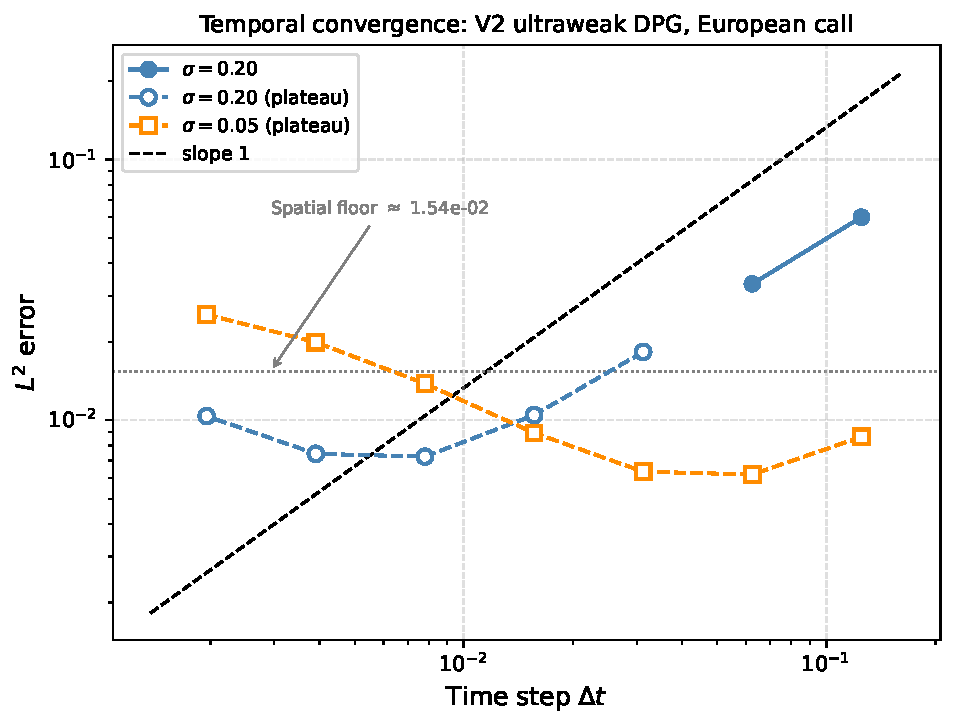
\includegraphics[width=0.72\textwidth]{figures/figN1_temporal_clean.pdf}
\caption{Log-log plot of $L^2$ error vs.\ $\dt$ for the Phase~N1
  temporal sweep.  Blue circles ($\sigma=0.20$): filled markers are
  pre-plateau (flag~0), dashed hollow markers are plateau (flag~1).
  Orange squares ($\sigma=0.05$): all hollow (all plateau).
  Black dashed line: reference slope~1.
  Gray dotted line: spatial floor $\eps_{\rm spatial} = 0.01535$.}
\label{fig:n1}
\end{figure}

Figure~\ref{fig:n1} shows that:
\begin{enumerate}[noitemsep]
\item The $\sigma=0.20$ curve follows the reference slope~1 closely
  for $\dt \in [0.016, 0.125]$ (i.e.\ $\Nt \in \{8,16,32,64\}$),
  confirming first-order temporal convergence.
\item Below $\dt \approx 0.008$ ($\Nt\ge128$), the $\sigma=0.20$
  curve deviates from slope~1: the error reaches a minimum and then
  increases, reflecting temporal--spatial error cancellation
  approaching the spatial floor.
\item The $\sigma=0.05$ curve lies entirely below the spatial floor
  at coarse $\dt$ and increases monotonically, demonstrating that
  the temporal error for low volatility is overwhelmed by the spatial
  floor throughout the sweep.
\end{enumerate}

% ==================================================================
\section{Discussion}
% ==================================================================

\subsection{Key findings}

\begin{enumerate}
\item \textbf{Backward Euler achieves first-order temporal convergence}
  for the V2 ultraweak DPG solver at $\sigma=0.20$.
  The fitted EOC of $0.85$ is slightly below the theoretical
  value of $1.0$; this bias arises because the spatial floor
  ($0.015$) is not negligible relative to the temporal error
  at the coarser time steps, adding a constant offset that
  reduces the apparent rate:
  \[
    \|e_h\|_{L^2} \approx C_t\,\dt + \eps_{\rm spatial}
    \;\;\Longrightarrow\;\;
    \text{apparent EOC} < 1.
  \]

\item \textbf{Temporal convergence is not demonstrable for
  $\sigma=0.05$} at $\Nx=256$.  The issue is that the
  temporal error constant $C_t$ for the convection-dominated
  regime is much smaller than for $\sigma=0.20$, so the spatial
  floor is never smaller than the temporal error within the
  sweep range.

\item \textbf{Preconditioner limitation.}  The V2 solver with
  \texttt{HypreAMS} failed silently for $\Nx > 300$.  Replacing
  with \texttt{HypreBoomerAMG} for the RT\_Trace block restores
  convergence at all tested mesh sizes.  Future work could
  explore a proper AMS setup for the trace space or an
  all-at-once space-time solver.
\end{enumerate}

\subsection{Recommendations for future studies}

\begin{itemize}[noitemsep]
\item To demonstrate $\bigo{\dt}$ convergence for $\sigma=0.05$,
  the spatial mesh must satisfy
  $\eps_{\rm spatial} \lesssim 10^{-3}$, requiring
  $\Nx \gtrsim 600$ and a more robust preconditioner.
\item Using a \emph{smooth} initial condition (e.g., starting from
  $\tau_0 = 0.1$ with the exact Black-Scholes solution as IC)
  would eliminate the kink-induced ATM oscillation at coarse $\dt$
  and expose cleaner temporal convergence rates even on moderate meshes.
\item The plateau detection criterion ($L^2 < 2\,\eps_{\rm spatial}$)
  is conservative: for $\sigma=0.20$, rows $\Nt=32,64$ show
  clear convergence (EOC $\approx 0.87,\,0.81$) but are
  classified as plateau.  A criterion based on observed EOC
  dropping below $0.5$ would be more physically meaningful.
\end{itemize}

% ==================================================================
\section{Files Produced}
% ==================================================================

\begin{center}
\begin{tabular}{ll}
\toprule
File & Description \\
\midrule
\texttt{results/convergence/v2\_temporal\_clean.csv}        & Sweep data, $\sigma=0.20$ \\
\texttt{results/convergence/v2\_temporal\_clean\_sigma005.csv} & Sweep data, $\sigma=0.05$ \\
\texttt{results/convergence/n1\_spatial\_floor.txt}         & Spatial floor record \\
\texttt{results/convergence/n1\_eoc\_summary.txt}            & Pre-plateau EOC summary \\
\texttt{results/figures/figN1\_temporal\_clean.pdf/.png}    & Figure N1 \\
\texttt{results/paper\_tables\_siam.tex}                     & \LaTeX\ table command \\
\texttt{results/paper\_text\_siam.tex}                       & \LaTeX\ text blurb \\
\texttt{scripts/run\_n1\_temporal.py}                        & Sweep driver \\
\texttt{scripts/plot\_n1\_temporal.py}                       & Figure generator \\
\texttt{scripts/generate\_table\_N1.py}                     & Table generator \\
\bottomrule
\end{tabular}
\end{center}

% ==================================================================
\appendix
\section{Solver Configuration Details}
% ==================================================================

\paragraph{JSON config used for each run.}
\begin{verbatim}
{
  "sigma": <sigma>, "r": 0.05, "T": 1.0, "K": 100.0,
  "x_min": -3.0,   "x_max": 3.0,
  "N_x": 256,      "N_t": <Nt>,
  "p": 2,          "delta_p": 1
}
\end{verbatim}
Each run is executed inside the Singularity container:
\begin{verbatim}
singularity exec --cleanenv --bind /path/to/repo:/workspace \
    /path/to/container/ \
    mpirun -np 4 /workspace/build/bin/main_european_1d_ultraweak_mpi \
    --config /workspace/config/<config>.json \
    --csv-path /workspace/results/convergence/<out>.csv
\end{verbatim}

\paragraph{Degrees of freedom at $\Nx=256$.}
\begin{center}
\begin{tabular}{lrr}
\toprule
Block & Space & Global DOFs \\
\midrule
$u_h$ (L2, $p-1=1$) & $L^2_{1}$ & 1\,024 \\
$\boldsymbol{\sigma}_h$ (L2$\times$2, $p-1=1$) & $[L^2_{1}]^2$ & 2\,048 \\
$\hat{u}_h$ (H1\_Trace, $p=2$) & $H^1_{\rm Trace}$ & (shared) \\
$\hat{f}_h$ (RT\_Trace, $p-1=1$) & $\mathrm{RT}_{\rm Trace}$ & (shared) \\
\cmidrule{2-3}
Total & & 5\,893 \\
\bottomrule
\end{tabular}
\end{center}

\end{document}
